
\chapter{2章のタイトル}
\label{chap:second}


\section{緒言}
本章では学内ゾーンにおける Elasticsearch クラスタへの
データ移行について述べる.

\section{概要}
今回は, ElasticSearchサーバー間でのデータ移行と, その際に行われた重複データの削除方法, kibanaによる可視化結果について報告する.

\section{データ移行手順について}

co2のデータ移行を行う上で, タイムスタンプと部屋番号の組み合わせが重複しているデータが一部存在しており, この重複データを取り除いた上でデータ移行を行う必要があったので, 一度, 移行元のElasticSearchサーバーのデータをローカルマシンにエクスポートして, 重複データを取り除いた上で, 移行先のElasticSearchサーバーにデータをアップロードした.

\subsection{データのエクスポート}
移行元のElasticSearchサーバーのデータのローカルマシンへのエクスポートには, elasticdumpライブラリを使用して, JSON形式でエクスポートした.その際, co2という文字列を含むインデックスのデータのみをエクスポートした.

\subsection{データの重複削除}
重複データの削除はSQLiteデータベースを用いて行った.

SQLiteデータベースはリレーショナルデータベースの一種であり, 複合主キーを使って複数のテーブルカラムの組み合わせを一意の識別子として扱うことができる. これにより, 同じ組み合わせのデータを重複して挿入しようとした場合, データベースエンジンがコンフリクトエラーを発生させ, 重複データの挿入を阻止する. そのため, 今回の重複データ削除には適していると判断した.

今回使用したSQLiteデータベースでは, 部屋番号(number)とタイムスタンプ(JPtime)を一意のキーとして設定した. 以下のリスト\ref{sc1}, リスト\ref{sc2}に示すように, 移行元のElasticSearchサーバーに保存されているco2インデックスのドキュメントは, フィールドのメンバーが統一されておらず, 一部センサー情報が存在しない場合がある. そのため, データの挿入時にコンフリクトエラーが発生した場合は, 既存のレコードと挿入しようとしたレコードを比較し, 既存レコードの値がNULLであるカラムにおいて, 挿入しようとしているレコードの値が非NULLである場合には, 既存レコードのカラムの値を更新するようにした. これにより, 重複データ削除時に一部センサー情報などが欠けてしまう問題を解決した.

\begin{lstlisting}[caption=\_sourceフィールドのメンバー数が少ないドキュメント, label=sc1]
{
  "_index": "co2_e411",
  "_type": "_doc",
  "_id": "nEi2nnoB2-iFXnrMOobM",
  "_score": 1,
  "_source": {
      "utctime": "2020-10-09T05:09:06+00:00",
      "number": "E411",
      "PPM": "481",
      "data": "Thingspeak"
  }
}
  \end{lstlisting}

\begin{lstlisting}[caption=\_sourceフィールドのメンバー数が多いドキュメント, label=sc2]
{
  "_index": "co2_e411",
  "_type": "_doc",
  "_id": "YKBqU4QBugDzeydA2gyi",
  "_score": 1,
  "_source": {
      "RH": 26.98,
      "PPM": 423,
      "JPtime": "2022-11-06T22:45:30.080925",
      "ip": "172.23.68.19/16",
      "utctime": "2022-11-06T13:45:30.080895",
      "TEMP": 24.47,
      "index_name": "co2_e411",
      "ms": "",
      "number": "E411"
  }
}
    \end{lstlisting}

\subsection{データのインポート}
重複データ削除後のデータが保存されたSQLiteテーブルからすべてのレコードを読み出して, ターゲットのElasticSearchサーバーに移行した.

その際, pythonのelasticsearchライブラリを使用し, タイムスタンプが2023年より以前のデータは2022\_co2という名前のインデックスに保存し, 2023年のものは2023\_co2という名前のインデックスに保存した.

\section{kibanaによるデータの可視化}

移行後のデータをkibanaを用いて可視化した.

2022\_co2インデックスと, 2023\_co2インデックスについて, 横軸をタイムスタンプとし, 縦軸をPPM, RH, TEMPとしてそれぞれプロットしたものを図 \ref{p1} 〜 図 \ref{p6}に示す.

\begin{figure}[!ht]
    \begin{center}
        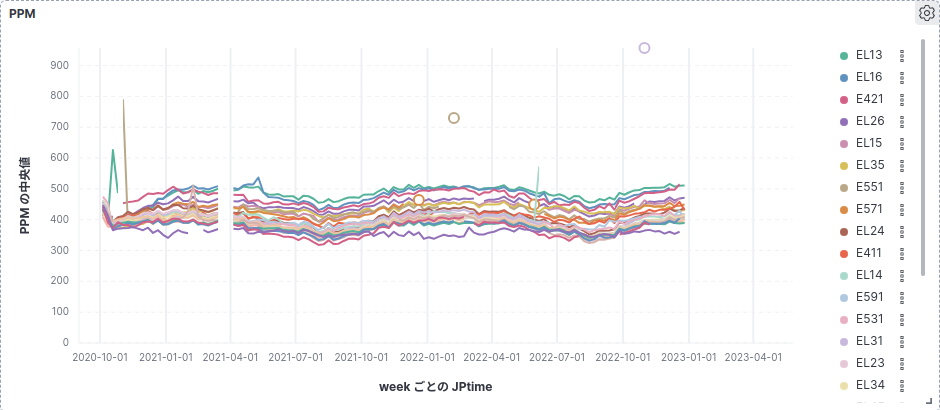
\includegraphics[width=160mm]{sotu/figure/2022_ppm.png}
        \caption{2022\_co2のPPM}
        \label{p1}
    \end{center}
\end{figure}

\begin{figure}[!ht]
    \begin{center}
        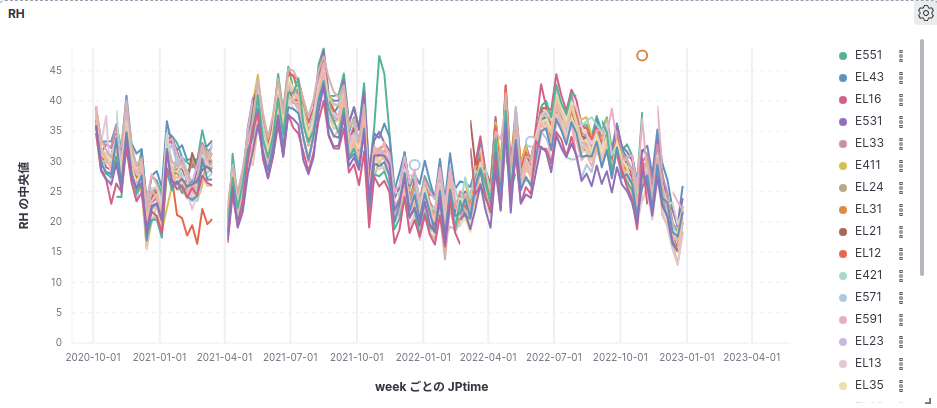
\includegraphics[width=160mm]{sotu/figure/2022_rh.png}
        \caption{2022\_co2のRH}
        \label{p2}
    \end{center}
\end{figure}

\begin{figure}[!ht]
    \begin{center}
        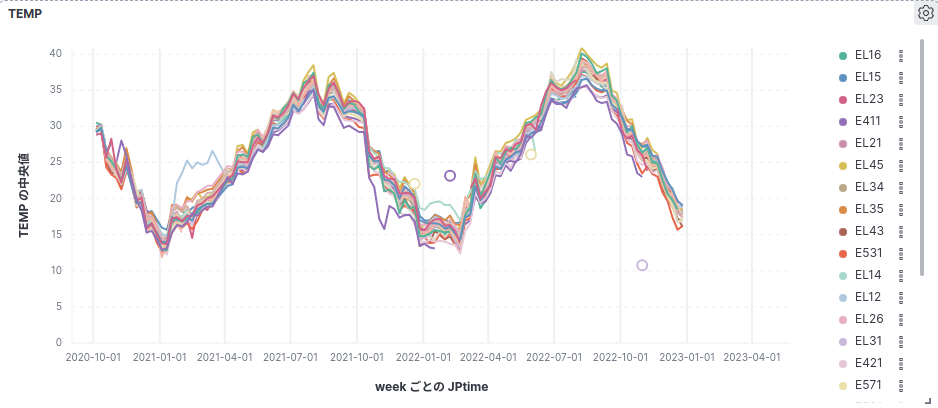
\includegraphics[width=160mm]{sotu/figure/2022_temp.png}
        \caption{2022\_co2のTEMP}
        \label{p3}
    \end{center}
\end{figure}

\begin{figure}[!ht]
    \begin{center}
        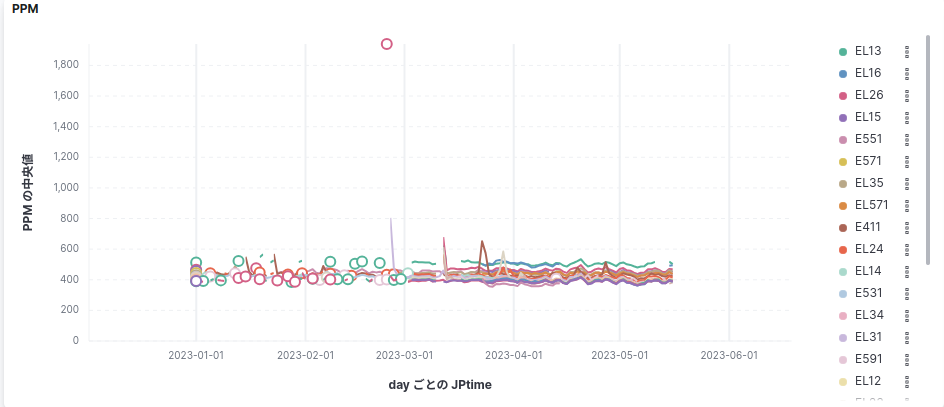
\includegraphics[width=160mm]{sotu/figure/2023_ppm.png}
        \caption{2023\_co2のPPM}
        \label{p4}
    \end{center}
\end{figure}

\begin{figure}[!ht]
    \begin{center}
        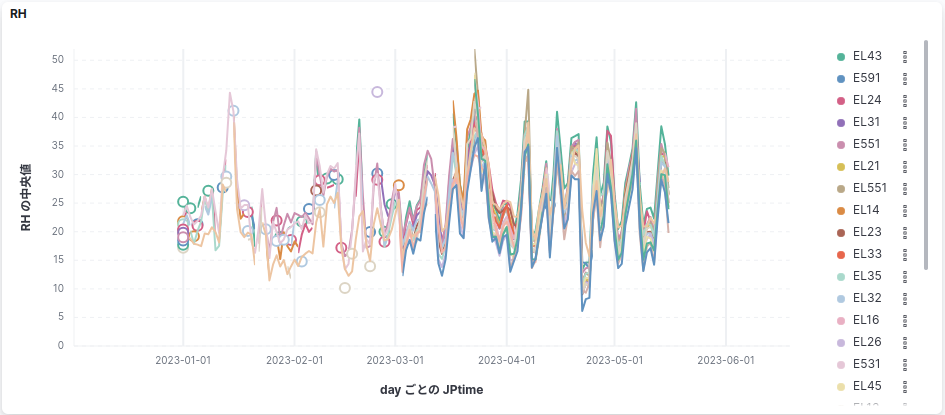
\includegraphics[width=160mm]{sotu/figure/2023_rh.png}
        \caption{2023\_co2のRH}
        \label{p5}
    \end{center}
\end{figure}

\begin{figure}[!ht]
    \begin{center}
        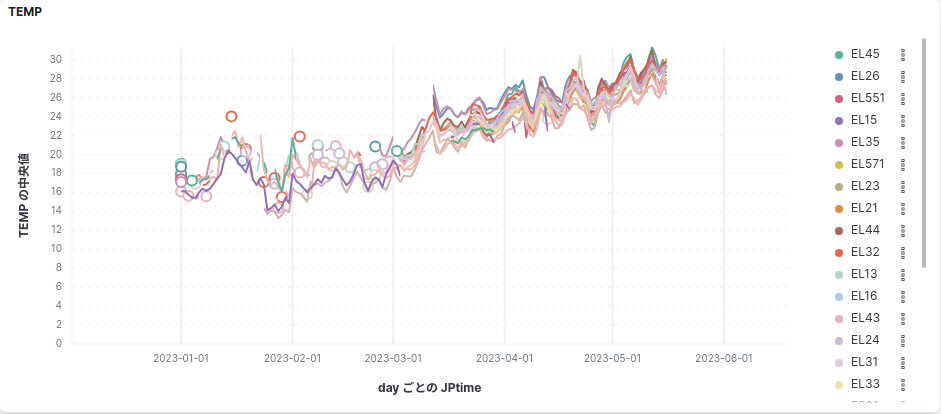
\includegraphics[width=160mm]{sotu/figure/2023_temp.png}
        \caption{2023\_co2のTEMP}
        \label{p6}
    \end{center}
\end{figure}

\section{概要}
今回は, 前回に引き続き133.71.106.168から133.71.106.141へのElasticSearchサーバー間のデータ移行とkibanaを用いた可視化結果について報告する.
また, 移行元ElasticSearchサーバーにあったCO\textsubscript{2}データ以外のデータの移行についても報告する.

\section{CO\textsubscript{2}データの移行作業}
前回の報告書では, 移行元ElasticSearchサーバーのCO\textsubscript{2}データについて, JPtimeが2023年より以前のドキュメントを2022\_co2という名前のインデックスに保存し, JPtimeが2023年のドキュメントを2023\_co2という名前のインデックスに保存した.
しかし, インデックスを分けることで2023年以前と2023年のデータをkibanaで同じグラフにプロットして確認することが難しい可能性があることと, ElasticSearchサーバー間のデータ移行が正しく完了したかkibanaで可視化することによって確認することが出来ないという問題があったため, 今回はJPtimeの値に関わらずco2という名前のインデックスに保存した.
保存先のインデックスがco2であることを除くと, データの移行手順は前回のものと同様の手順で行った.

\section{kibanaによるデータの可視化}

移行後のco2インデックスに保存されたデータをkibanaを用いて可視化した.

横軸をタイムスタンプとし, 縦軸をPPM, RH, TEMPとしてそれぞれプロットしたものを図 \ref{p7} 〜 図 \ref{p9}に示す.

\begin{figure}[!ht]
    \begin{center}
        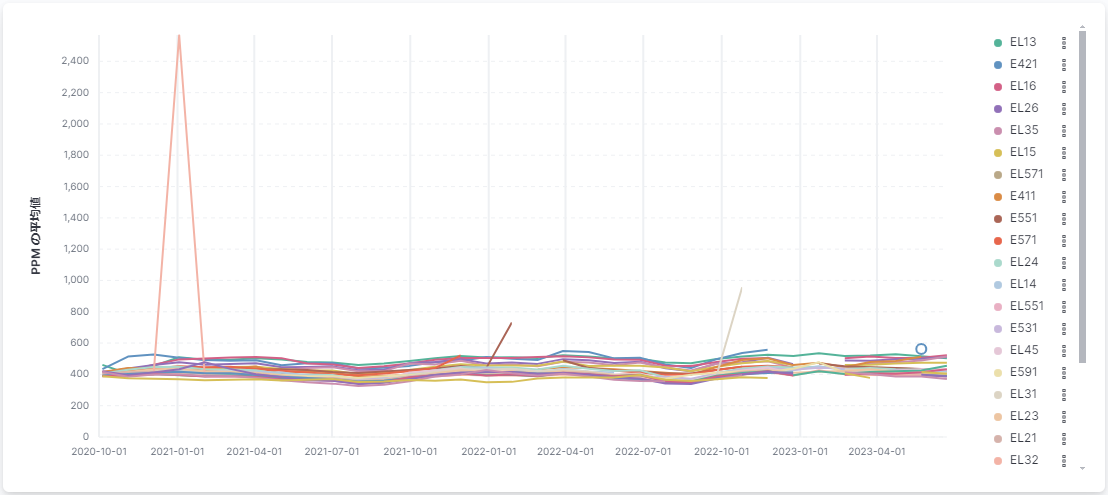
\includegraphics[width=160mm]{sotu/figure/ppm.png}
        \caption{co2のPPM}
        \label{p7}
    \end{center}
\end{figure}

\begin{figure}[!ht]
    \begin{center}
        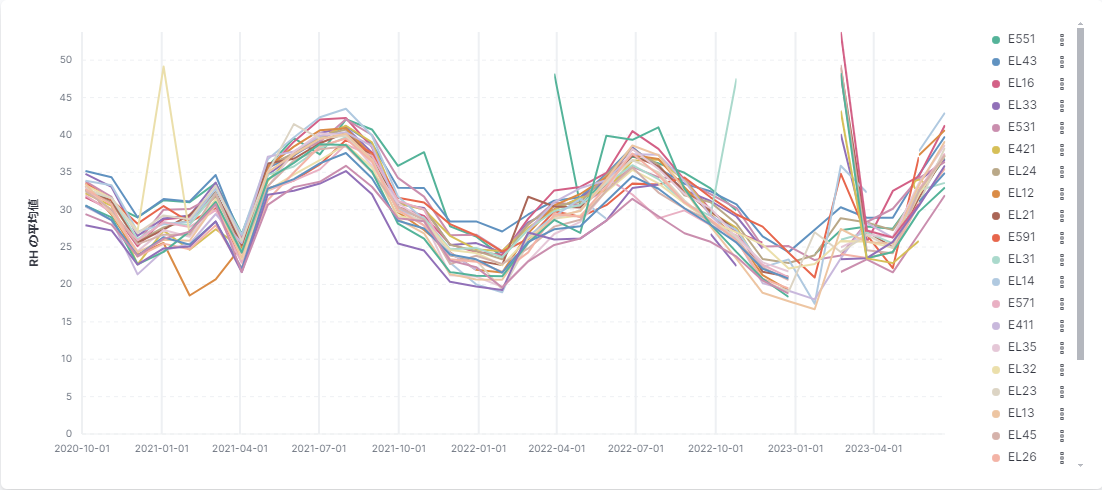
\includegraphics[width=160mm]{sotu/figure/rh.png}
        \caption{co2のRH}
        \label{p8}
    \end{center}
\end{figure}

\begin{figure}[!ht]
    \begin{center}
        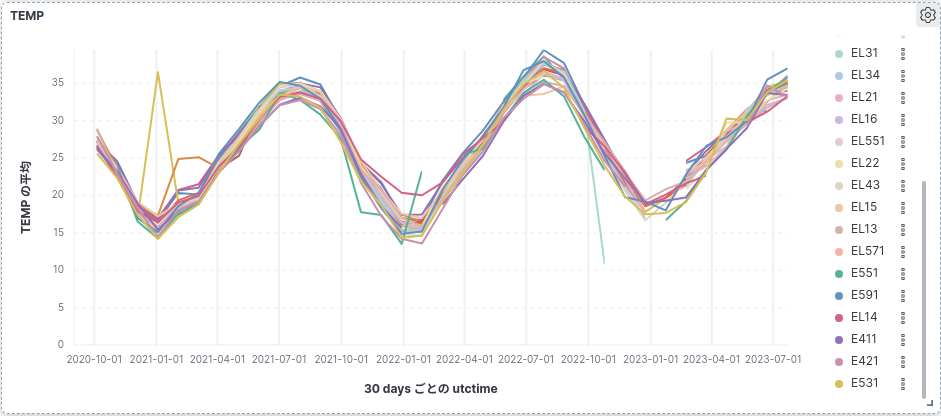
\includegraphics[width=160mm]{sotu/figure/temp.png}
        \caption{co2のTEMP}
        \label{p9}
    \end{center}
\end{figure}

図 \ref{p7} 〜 図 \ref{p9}について, 2022年と2023年の境目でデータが連続的に変化していることが確認出来るので, データ移行作業は正常に行うことが出来たと判断できる.

\section{CO\textsubscript{2}データ以外のデータの移行について}

移行元のElasticSearchサーバーにはインデックス名にco2という文字列を含むインデックス以外に以下のインデックスがあった.

\begin{itemize}
    \item movement\_diary
    \item movement\_diary01
    \item temp2
    \item temp3
    \item test
\end{itemize}

これらのインデックスのデータ移行は, 同名のインデックスを移行先のElasticSearchサーバーに作成して, 作成したインデックスにデータを挿入することで行った.

ただし, testインデックスは移行先のElasticSearchサーバーに既に同名のインデックスが作成されていたので, 133.71.106.168\_testというインデックス名にした.

次に, 上記のインデックスに保存されているデータについて説明する.

temp2, temp3はTIME, TEMP, HUMIフィールドを持ったドキュメントが格納されており, temp2のドキュメント数は約150件, temp3は約60件であった.
testはJPtime, PPM, RH, TEMP, ip, number, utctimeフィールドを持ったドキュメントを格納しているインデックスであり, ドキュメント数は95件であった.
これらの情報から, temp2, temp3, testインデックスはCO\textsubscript{2}データの収集の研究の中で動作確認目的に作成されたインデックスではないかと考えられる.

% movement\_diaryとmovement\_diary01は運行日誌に関する情報を格納したインデックスであり, それぞれ以下のような構造のドキュメントが保存されている.

% \begin{lstlisting}[caption=movement\_diaryのドキュメントデータ, label=sc3]
%   {
%     "_index": "movement_diary",
%     "_type": "_doc",
%     "_id": "OL65VHwBr1DnHOWC_d0U",
%     "_score": 1.0,
%     "_source": {
%         "pageNo": "1",
%         "type": "運行日誌",
%         "wether": "雨",
%         "driver": "仲村泰明",
%         "passenger": 2,
%         "destination": "新田高校・松山聖稜高校",
%         "dt_S": "2018-05-08T08:26:00",
%         "battery_S": 99,
%         "cruisingdistance_S": null,
%         "odometer_S": 15,
%         "out_charge": "していない",
%         "etc": "使用していない",
%         "etc_section": "",
%         "etc_budget": "",
%         "dt_R": "2018-05-08T11:50:00",
%         "battery_R": 94,
%         "cruisingdistance_AC": null,
%         "odometer_R": 30.0,
%         "meter": 15.0,
%         "start_charg_time": "2018-05-08T11:52:00",
%         "remark": "感じなかった",
%         "inspection": null,
%         "break_rest_Be": null,
%         "break_rest_Af": null,
%         "tire_rest_Be": null,
%         "tire_rest_Af": null,
%         "inspection_battery": null,
%         "charging_rate": null,
%         "health": null
%     }
% }
% \end{lstlisting}

% \begin{lstlisting}[caption=movement\_diary01のドキュメントデータ, label=sc4]
%   {
%     "_index": "movement_diary01",
%     "_type": "_doc",
%     "_id": "oMmqbnwBr1DnHOWCgH9O",
%     "_score": 1.0,
%     "_source": {
%         "pageNo": "1",
%         "type": "運行日誌",
%         "wether": "雨",
%         "driver": [
%             "仲村泰明",
%             null,
%             null
%         ],
%         "destination": [
%             "新田高校",
%             "松山聖稜高校"
%         ],
%         "dt_S": "2018-05-08T08:26:00",
%         "battery_S": 99,
%         "cruisingdistance_S": null,
%         "odometer_S": 15,
%         "out_charge": "していない",
%         "charge_place": "",
%         "etc": "使用していない",
%         "etc_section": "",
%         "etc_budget": "",
%         "dt_R": "2018-05-08T11:50:00",
%         "battery_R": 94,
%         "cruisingdistance_AC": null,
%         "odometer_R": 30.0,
%         "meter": 15.0,
%         "start_charg_time": "2018-05-08T11:52:00",
%         "remark": "感じなかった",
%         "inspection": null,
%         "break_rest_Be": null,
%         "break_rest_Af": null,
%         "tire_rest_Be": null,
%         "tire_rest_Af": null,
%         "inspection_battery": null,
%         "charging_rate": null,
%         "health": null,
%         "battery_rate": 5,
%         "battery_rate_distance": 3.0
%     }
% }
% \end{lstlisting}

以下にmovement\_diaryとmovement\_diary01のドキュメントの違いを列挙する.

\begin{enumerate}
    \item driverフィールド:
          \begin{itemize}
              \item movement\_diaryのドキュメントでは, driverフィールドは文字列である.
              \item movement\_diary01のドキュメントでは, driverフィールドは配列で, その中に文字列と2つのnull値が含まれている.
          \end{itemize}
          
    \item ``destination''フィールド:
          \begin{itemize}
              \item movement\_diaryのドキュメントでは, ``destination''フィールドは単一の文字列である.
              \item movement\_diary01のドキュメントでは, ``destination''フィールドは配列で, その中に2つの文字列が含まれている.
          \end{itemize}
          
    \item ``charge\_place''フィールド:
          \begin{itemize}
              \item movement\_diaryのドキュメントには, ``charge\_place''フィールドは存在しない.
              \item movement\_diary01のドキュメントでは, ``charge\_place''フィールドが追加されているが, その値は空文字列である.
          \end{itemize}
          
    \item ``battery\_rate''フィールド:
          \begin{itemize}
              \item movement\_diaryのドキュメントには, ``battery\_rate''フィールドは存在しない.
              \item movement\_diary01のドキュメントでは, ``battery\_rate''フィールドが追加されており, その値は数値である.
          \end{itemize}
          
    \item ``battery\_rate\_distance''フィールド:
          \begin{itemize}
              \item movement\_diaryのドキュメントには, ``battery\_rate\_distance''フィールドは存在しない.
              \item movement\_diary01のドキュメントでは, ``battery\_rate\_distance''フィールドが追加されており, その値は数値である.
          \end{itemize}
          
\end{enumerate}

\section{概要}
今回は, 133.71.201.197から133.71.106.141へのElasticSearchサーバー間のリサイクル館の太陽光パネルの測定データ移行とkibanaを用いた可視化結果について報告する.
また, 133.71.106.168のElasticSearchサーバーにあったmovement\_diaryインデックスとmovement\_diary01インデックスのドキュメントについて調査した結果も報告する.

\section{データ移行手順について}

データ移行を行う上で, ローカルマシンにJSON形式でダンプしていたデータと, 133.71.201.197のElasticSearchサーバー上に存在するデータとの間で重複しているデータが一部存在しており, この重複データを取り除いた上でデータ移行を行う必要があった.

そこで一度, 移行元のElasticSearchサーバーのデータをローカルマシンにエクスポートして, 重複データを取り除いた上で, 移行先のElasticSearchサーバーにデータをアップロードした.

\subsection{データのエクスポート}
移行元のElasticSearchサーバーのデータのローカルマシンへのエクスポートには, elasticdumpライブラリを使用してJSON形式でエクスポートした.その際, pcs\_recyclekanという名前のインデックスのデータをエクスポートした.

\subsection{データの重複削除}
重複データの削除は, 予めローカルマシンにJSON形式でダンプしていたデータと, elasticdumpライブラリを使用してJSON形式でエクスポートしたデータを, utctimeフィールドの値がユニークになるようにフィルタリングすることで行った.

\subsection{データのインポート}
重複データ削除後のデータを保存したJSONファイルを読み出して, 移行先のElasticSearchサーバーにアップロードした.

その際, pythonのelasticsearchライブラリを使用し,133.71.201.197のElasticSearchサーバーと同名のpcs\_recyclekanという名前のインデックスに保存した.

\section{kibanaによるデータの可視化}

移行後のpcs\_recyclekanインデックスに保存されたデータをkibanaを用いて可視化した.

% 横軸をタイムスタンプ(JPtime)とし, 縦軸を日射量(solarIrradiance(\si{kw/m^2}))としてプロットしたものを図 \ref{p10}に示す.

\begin{figure}[!ht]
    \begin{center}
        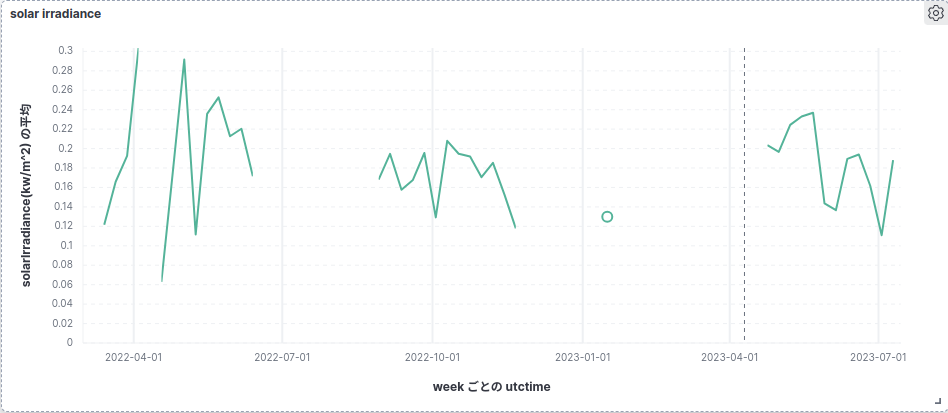
\includegraphics[width=160mm]{sotu/figure/1.png}
        \caption{133.71.106.141のpcs\_recyclekan}
        \label{p10}
    \end{center}
\end{figure}

次に, 移行元である133.71.201.197のElasticSearchサーバーのpcs\_recyclekanインデックスに保存されたデータを図 \ref{p2}に示す.

\begin{figure}[!ht]
    \begin{center}
        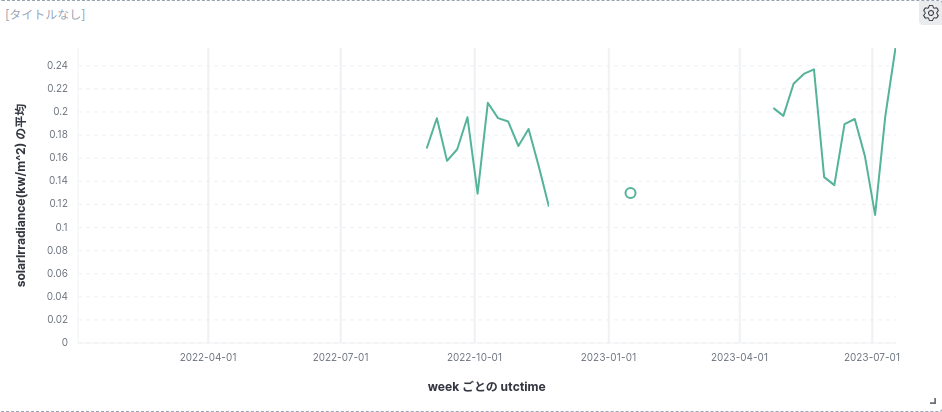
\includegraphics[width=160mm]{sotu/figure/2.png}
        \caption{133.71.201.197のpcs\_recyclekan}
        \label{p11}
    \end{center}
\end{figure}

図 \ref{p10}, 図 \ref{p11}について, 2022年8月以降のグラフの概形が一致していることが確認出来るので, データ移行作業は正常に行うことが出来たと判断できる.

\section{movement\_diaryのデータについて}
movement\_diaryとmovement\_diary01はデータ型が異なる一部のフィールドを除いて全て同じデータを保有しており, それぞれのインデックスのドキュメント数の比較と, タイムスタンプ情報を格納するフィールドのインデックス間での比較を行うことで, movement\_diaryが不要なインデックスであるかを調査した.

まず, movement\_diaryとmovement\_diary01のドキュメント数を調べたところ, 同じ142件であった.

次に, movement\_diaryとmovement\_diary01でタイムスタンプ情報を持つフィールドであるdt\_Sフィールドの値同士を比較した.

ただし, dt\_Sフィールドがnullのドキュメントが一部存在するので, その場合はタイムスタンプ情報を持つinspectionフィールドの値同士を比較した.

比較した結果, dt\_Sフィールドとinspectionフィールドの両方がnullである3件のドキュメントを除いて他全てのドキュメントはdt\_Sフィールドもしくはinspectionフィールドの値がmovement\_diaryとmovement\_diary01の間で一致した.

dt\_Sフィールドとinspectionフィールドの両方がnullだった3件のドキュメントについても, 全てのフィールドにおいて, movement\_diary01のドキュメントがmovement\_diaryのドキュメントの持つ情報を持っていたので, これらの調査結果からmovement\_diaryインデックスはmovement\_diary01インデックスで代替でき, 削除して良いインデックスであると判断した.


\section{概要}
今回は, 133.71.201.197から133.71.106.141へのElasticSearchサーバー間のCO\textsubscript{2}データの移行後に発生したラズベリーパイからデータのインサートが出来ない問題への対応と, 移行元ElasticSearchサーバーから移行されていないCO\textsubscript{2}データの移行について報告する.

\section{ラズベリーパイからデータのインサートが出来ない問題について}

私が実装したデータ移行プログラムを使用して作成したElasticSearchのインデックスに対してラズベリーパイからデータのインサートが出来ない問題が発生した.

そこで, インデックスの作成を私のデータ移行プログラム上からではなく, 高木君側で行ってもらい, ラズベリーパイから正常にデータのインサートが出来ていることを確認した上で, 私が実装したデータ移行プログラムを使用してCO\textsubscript{2}データの移行を行うことで問題を解決した.

\section{移行元ElasticSearchサーバーから移行されていないCO\textsubscript{2}データの移行について}

私が実装したデータ移行プログラムを使用して133.71.201.197から133.71.106.141のElasticSearchサーバーへCO\textsubscript{2}データを移行したのが2023年5月中旬頃であり, 高木君が, 移行先である133.71.106.141のElasticSearchサーバーに対してラズベリーパイからCO\textsubscript{2}データのインサートを行うよう対応したのが2023年7月中旬であったため, 2023年5月中旬から2023年7月中旬までの間の約2ヶ月間のCO\textsubscript{2}データが移行先のElasticSearchサーバーに移行出来ていなかった. そこで, 追加の移行作業を行った.

移行方法は以下のとおりである.

\begin{enumerate}
    \item まず, 2023年5月中旬に移行した際の全移行データの中で最も最新のutctimeフィールドの値を検索する.
          \begin{itemize}
              \item 検索した結果, 2023年5月中旬に移行した際の全移行データの中で最も最新のutctimeは「2023-05-16T05:48:30.081305」であった.
          \end{itemize}
    \item 次に, 移行先ElasticSearchサーバーに対してラズベリーパイからインサートされた全データの中で最も古いutctimeフィールドの値を検索する.
          \begin{itemize}
              \item 検索した結果, ラズベリーパイからインサートされた全データの中で最も古いutctimeは「2023-07-20T07:15:39.314008」であった.
          \end{itemize}
    \item 前回のCO\textsubscript{2}データの移行は2023年5月中旬頃に行ったため, 2023年5月1日0時0分0秒以降のutctimeを持つドキュメントを, 移行元ElasticSearchサーバーのインデックス名にco2という文字列を含むインデックスからelasticdump \cite{1}ライブラリを使用してローカルマシンにエクスポートする.
    \item 部屋番号(number)とタイムスタンプ(JPtime)の組み合わせがユニークになるようにエクスポートしたデータをフィルタリングする.
    \item 更に, 1と2で得られたutctimeの範囲に含まれるutctimeを持つドキュメントのみになるようフィルタリングする.
    \item フィルタリング後のデータを移行先ElasticSearchサーバーにバルクインサートする.
\end{enumerate}

\section{kibanaによるデータの可視化}

2023年5月中旬から2023年7月中旬までの間の約2ヶ月間のCO\textsubscript{2}データを移行した後のco2\_modbusインデックスについて, 横軸をタイムスタンプ(utctime)とし, 縦軸をPPM, RH, TEMPとしてそれぞれプロットしたものを図 \ref{p12} 〜 図 \ref{p14}に示す.

\begin{figure}[!ht]
    \begin{center}
        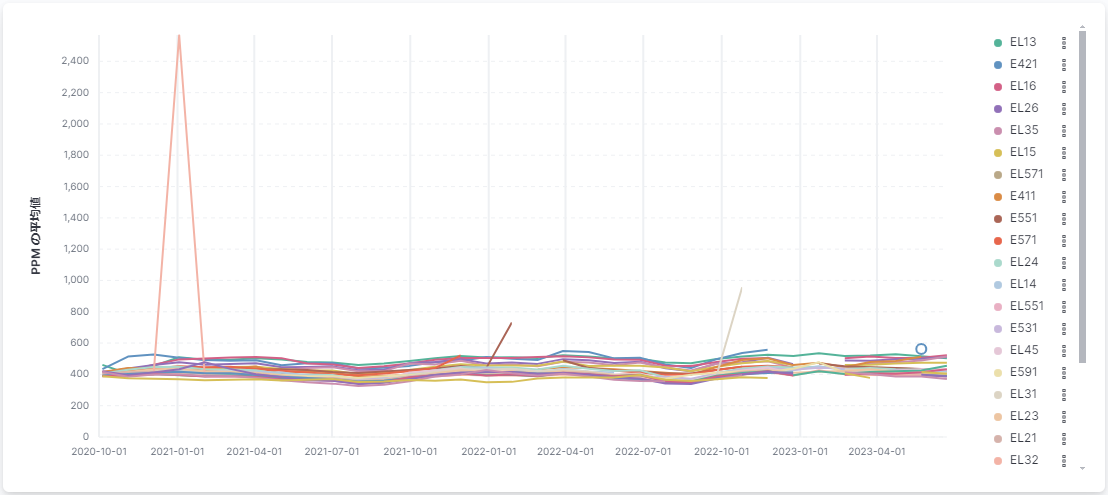
\includegraphics[width=160mm]{sotu/figure/ppm.png}
        \caption{co2\_modbusのPPM}
        \label{p12}
    \end{center}
\end{figure}

\begin{figure}[!ht]
    \begin{center}
        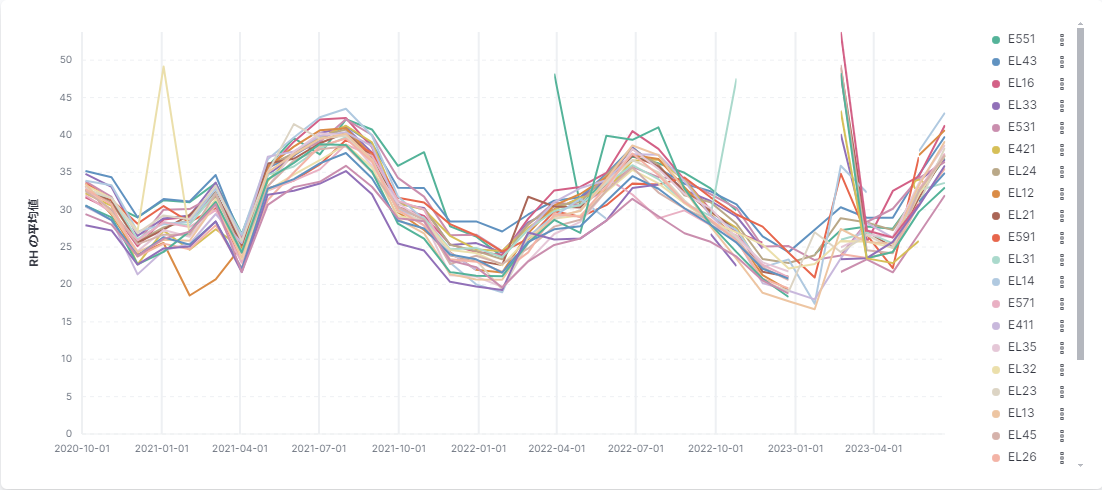
\includegraphics[width=160mm]{sotu/figure/rh.png}
        \caption{co2\_modbusのRH}
        \label{p13}
    \end{center}
\end{figure}

\begin{figure}[!ht]
    \begin{center}
        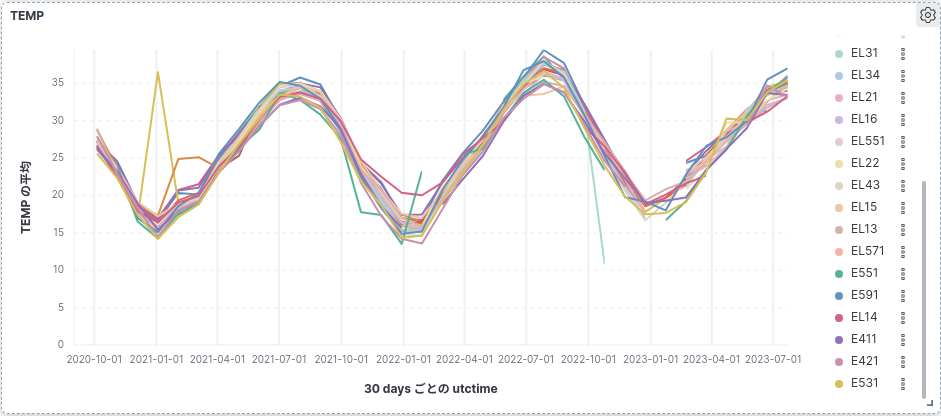
\includegraphics[width=160mm]{sotu/figure/temp.png}
        \caption{co2\_modbusのTEMP}
        \label{p14}
    \end{center}
\end{figure}

今回, 追加でCO\textsubscript{2}データを移行した2023年5月中旬から2023年7月中旬までの期間とその前後の期間において, 図 \ref{p12} 〜 図 \ref{p14}より, 連続的にデータが変化していることが目視で確認できるので, データ移行は正常に出来たと判断できる.


\section{概要}
今回は, 133.71.201.197のElasticSearchサーバーにあるpcs\_recyclekanという名前のインデックス以外のインデックスについて調査を行い, 133.71.106.141のElasticSearchサーバーにデータ移行を行ったことについて報告する.

\section{133.71.201.197のElasticSearchサーバーにあるインデックスについて}
図 \ref{p15}に133.71.201.197のElasticSearchサーバーにあるインデックスの一覧を示す.

\begin{figure}[!ht]
    \begin{center}
        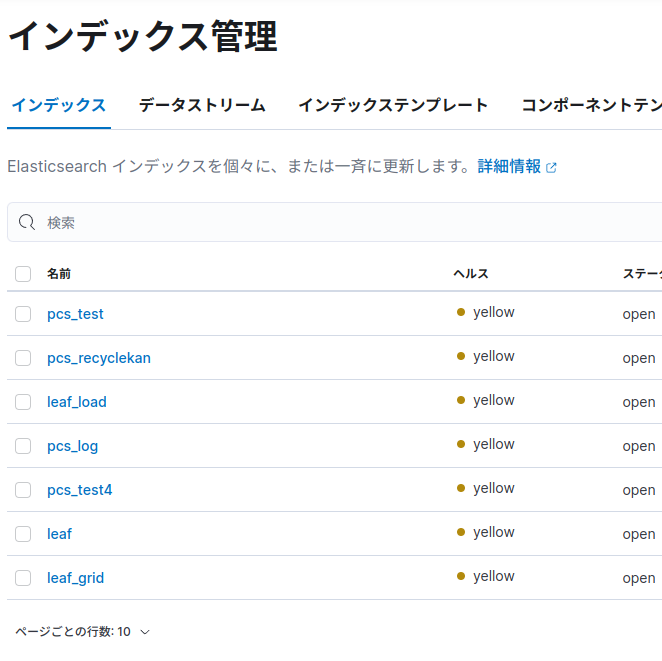
\includegraphics[width=160mm]{sotu/figure/indexes.png}
        \caption{133.71.201.197のElasticSearchサーバーにあるインデックスの一覧}
        \label{p15}
    \end{center}
\end{figure}

これらのインデックスが保存しているデータについて説明する.

\begin{itemize}
    \item pcs\_test
          \begin{itemize}
              \item 恵村君がプログラムの検証目的で使用しているインデックス
          \end{itemize}
    \item pcs\_recyclekan
          \begin{itemize}
              \item リサイクル館の太陽光発電に関するデータを保存しているインデックス
          \end{itemize}
    \item leaf\_load
          \begin{itemize}
              \item leafのデータが保存されているインデックス
          \end{itemize}
    \item pcs\_log
          \begin{itemize}
              \item リサイクル館の太陽光発電に関するデータをElasticSearchにインサートするPythonプログラムのログ情報を保存しているインデックス
          \end{itemize}
    \item pcs\_test4
          \begin{itemize}
              \item 恵村君がプログラムの検証目的で使用しているインデックス
          \end{itemize}
    \item leaf
          \begin{itemize}
              \item leafのデータが保存されているインデックス
          \end{itemize}
    \item leaf\_grid
          \begin{itemize}
              \item leafのデータが保存されているインデックス
          \end{itemize}
\end{itemize}

なお, leaf, leaf\_grid, leaf\_loadインデックスについて, Kibanaで各インデックスのマッピング情報を確認したところ, 3つともすべて同じマッピング情報を保持しており, 同じフィールドを持つドキュメントをそれぞれのインデックスで保存していることが分かった.

% leaf, leaf\_grid, leaf\_loadインデックスのマッピング情報をリスト\ref{sc5}に示す.

% \begin{lstlisting}[caption=leafと名の付くインデックスが持つマッピング情報,label=sc5]
%   {
%     "mappings": {
%       "_doc": {
%         "properties": {
%           "@timestamp": {
%             "type": "date"
%           },
%           "A1": {
%             "type": "float"
%           },
%           "A2": {
%             "type": "float"
%           },
%           "F": {
%             "type": "float"
%           },
%           "JPtime": {
%             "type": "date"
%           },
%           "P": {
%             "type": "float"
%           },
%           "P1": {
%             "type": "float"
%           },
%           "P2": {
%             "type": "float"
%           },
%           "PF": {
%             "type": "float"
%           },
%           "PF1": {
%             "type": "float"
%           },
%           "PF2": {
%             "type": "float"
%           },
%           "Q": {
%             "type": "float"
%           },
%           "Q1": {
%             "type": "float"
%           },
%           "Q2": {
%             "type": "float"
%           },
%           "S": {
%             "type": "float"
%           },
%           "S1": {
%             "type": "float"
%           },
%           "S2": {
%             "type": "float"
%           },
%           "V1": {
%             "type": "float"
%           },
%           "V2": {
%             "type": "float"
%           },
%           "data_time": {
%             "type": "date"
%           },
%           "type": {
%             "type": "text",
%             "fields": {
%               "keyword": {
%                 "type": "keyword",
%                 "ignore_above": 256
%               }
%             }
%           }
%         }
%       }
%     }
%   }
% \end{lstlisting}

pcs\_testインデックスとpcs\_test4インデックスに関しては, 恵村君が検証用途で使用しているものであるため, 今回の移行対象からは除外し, pcs\_log, leaf, leaf\_load, leaf\_gridインデックスのみを移行対象とした.

\section{データ移行手順について}

データ移行手順について, まず移行元のElasticSearchサーバーのデータをローカルマシンにJSON形式でエクスポートして, 作成したPythonプログラムを実行して移行先のElasticSearchサーバーにデータをインサートした.

\subsection{データのエクスポート}
移行元のElasticSearchサーバーのデータのローカルマシンへのエクスポートには, elasticdump \cite{1}ライブラリを使用してJSON形式でエクスポートした.その際, pcs\_log, leaf, leaf\_load, leaf\_gridという名前のインデックスのデータをエクスポートした.

\subsection{データのインポート}
エクスポートしたJSONファイルを, 作成したPythonプログラムから読み込んで, Pythonのelasticsearchライブラリを用いて移行先のElasticSearchサーバーにインサートした.

移行先のElasticSearchサーバーにおけるインデックス名については, 133.71.201.197のElasticSearchサーバーと同名のインデックスに保存した.

\section{データ移行が正常に行えたか確認}
図 \ref{p16}に移行元のElasticSearchサーバーのleafという文字列を含むインデックスのドキュメント数をカウントしたものを, 図 \ref{p3}に移行先のElasticSearchサーバーのleafという文字列を含むインデックスのドキュメント数をカウントしたものを示す.

図 \ref{p16}と図 \ref{p17}より, ドキュメント数が一致していることからデータ移行が正常に行えたと判断できる.

\begin{figure}[!ht]
    \begin{center}
        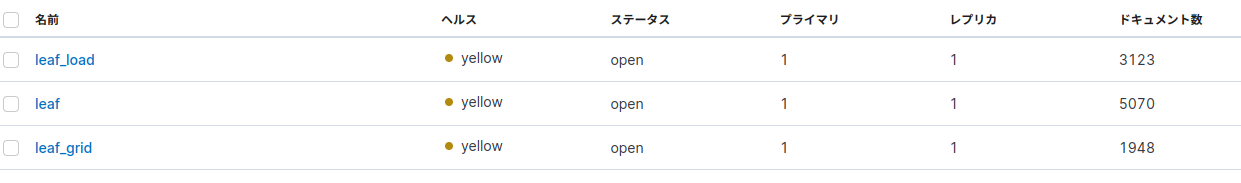
\includegraphics[width=160mm]{sotu/figure/197leaf.png}
        \caption{133.71.201.197のElasticSearchサーバーのleafという文字列を含むインデックスのドキュメントのカウント結果}
        \label{p16}
    \end{center}
\end{figure}

\begin{figure}[!ht]
    \begin{center}
        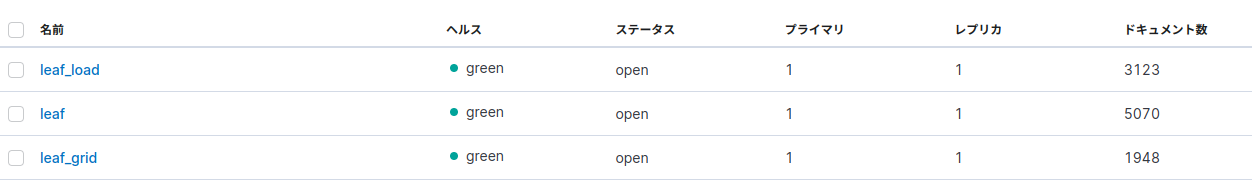
\includegraphics[width=160mm]{sotu/figure/141leaf.png}
        \caption{133.71.106.141のElasticSearchサーバーのleafという文字列を含むインデックスのドキュメントのカウント結果}
        \label{p17}
    \end{center}
\end{figure}

次に, 図 \ref{p18}に移行元のElasticSearchサーバーのpcs\_logインデックスのドキュメント数をカウントしたものを, 図 \ref{p5}に移行先のElasticSearchサーバーのpcs\_logインデックスのドキュメント数をカウントしたものを示す.

図 \ref{p18}と図 \ref{p19}より, ドキュメント数が一致していることからデータ移行が正常に行えたと判断できる.

\begin{figure}[!ht]
    \begin{center}
        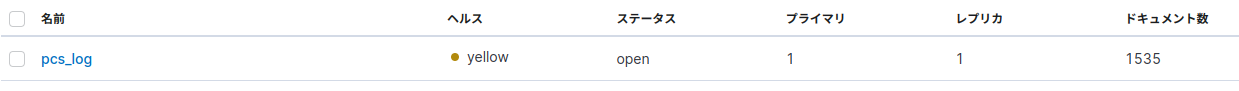
\includegraphics[width=160mm]{sotu/figure/197pcs.png}
        \caption{133.71.201.197のElasticSearchサーバーのpcs\_logインデックスのドキュメントのカウント結果}
        \label{p18}
    \end{center}
\end{figure}

\begin{figure}[!ht]
    \begin{center}
        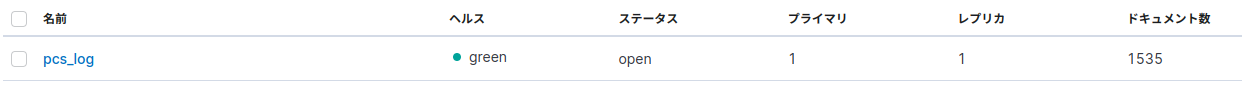
\includegraphics[width=160mm]{sotu/figure/141pcs.png}
        \caption{133.71.106.141のElasticSearchサーバーのpcs\_logインデックスのドキュメントのカウント結果}
        \label{p19}
    \end{center}
\end{figure}

\section{概要}
今回は, CO\textsubscript{2}データの収集を行っているラズベリーパイの一部が, データ移行作業の移行先である133.71.106.141のElasticSearchサーバーのco2インデックスに対してインサートを行っていたことにより, 正しいデータ移行先であるco2\_modbusインデックス以外のインデックスに一部のCO\textsubscript{2}データが保存されている問題を解消したことについて報告する.

\section{データ移行手順について}

ラズベリーパイからco2インデックスに対してインサートした全てのドキュメントをローカルマシンにJSON形式でエクスポートした後, 作成したPythonプログラムを実行してco2\_modbusインデックスにインサートした.

\subsection{データのエクスポート}
移行元のElasticSearchサーバーのデータのローカルマシンへのエクスポートには, elasticdump \cite{1}ライブラリを使用してJSON形式でエクスポートした.

co2インデックスに対してラズベリーパイからインサートしたデータにはJPtimeフィールドが存在しないため, JPtimeフィールドが存在しないドキュメントのみを対象としてエクスポートした.

また, エクスポートしたJSONデータを解析したところ, 最も古いutctimeフィールドの日付は2023年7月5日だった.

\subsection{データのインポート}
エクスポートしたJSONファイルを, 作成したPythonプログラムから読み込み, Pythonのelasticsearchライブラリを用いてco2\_modbusインデックスにインサートした.

\section{データ移行が正常に行えたか確認}
図 \ref{p20}にco2インデックスの2023年7月1日以降のPPM値の推移をグラフにしたものを, 図 \ref{p3}にco2\_modbusインデックスの2023年7月1日以降のPPM値の推移をグラフにしたものを示す.

図 \ref{p20}と図 \ref{p21}より, co2インデックスのデータが正常にco2\_modbusインデックスに移行できていることが分かる.

\begin{figure}[!ht]
    \begin{center}
        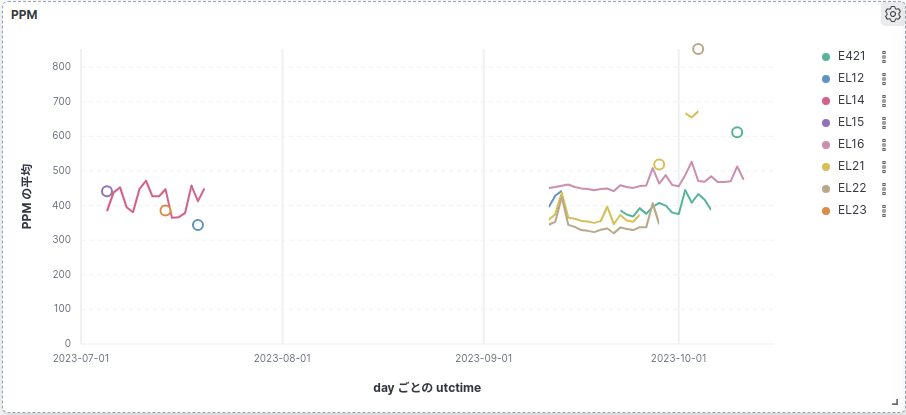
\includegraphics[width=160mm]{sotu/figure/co2PPM.png}
        \caption{co2インデックスのPPM}
        \label{p20}
    \end{center}
\end{figure}

\begin{figure}[!ht]
    \begin{center}
        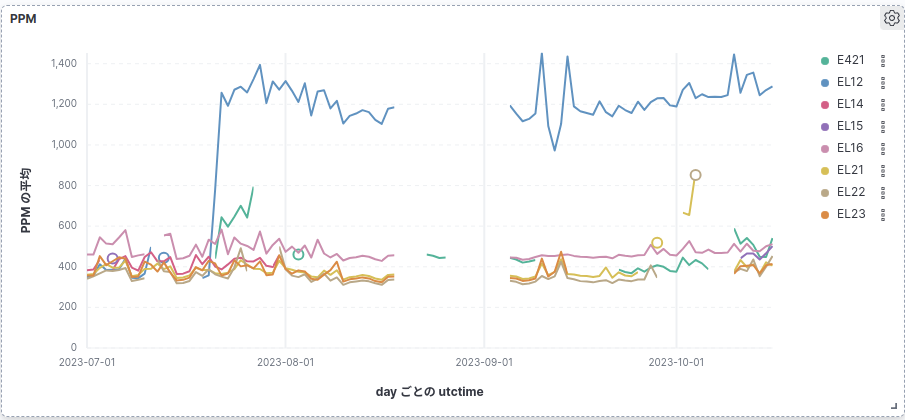
\includegraphics[width=160mm]{sotu/figure/co2ModbusPPM.png}
        \caption{co2\_modbusインデックスのPPM}
        \label{p21}
    \end{center}
\end{figure}

次に, 図 \ref{p22}にco2インデックスの2023年7月1日以降のRH値の推移をグラフにしたものを, 図 \ref{p5}にco2\_modbusインデックスの2023年7月1日以降のRH値の推移をグラフにしたものを示す.

図 \ref{p22}と図 \ref{p23}より, co2インデックスのデータが正常にco2\_modbusインデックスに移行できていることが分かる.

\begin{figure}[!ht]
    \begin{center}
        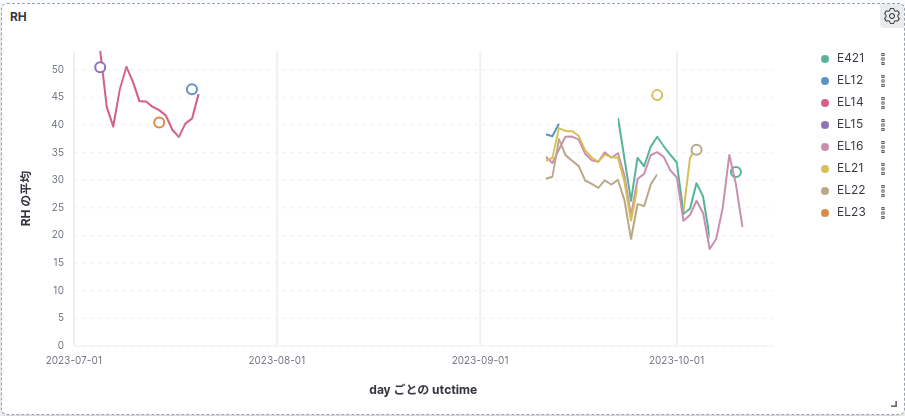
\includegraphics[width=160mm]{sotu/figure/co2RH.png}
        \caption{co2インデックスのRH}
        \label{p22}
    \end{center}
\end{figure}

\begin{figure}[!ht]
    \begin{center}
        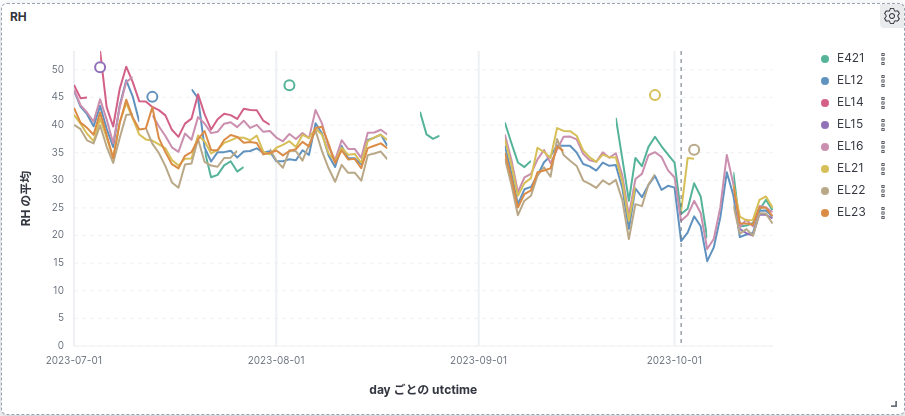
\includegraphics[width=160mm]{sotu/figure/co2ModbusRH.png}
        \caption{co2\_modbusインデックスのRH}
        \label{p23}
    \end{center}
\end{figure}

次に, 図 \ref{p24}にco2インデックスの2023年7月1日以降のTEMP値の推移をグラフにしたものを, 図 \ref{p28}にco2\_modbusインデックスの2023年7月1日以降のTEMP値の推移をグラフにしたものを示す.

図 \ref{p24}と図 \ref{p28}より, co2インデックスのデータが正常にco2\_modbusインデックスに移行できていることが分かる.

\begin{figure}[!ht]
    \begin{center}
        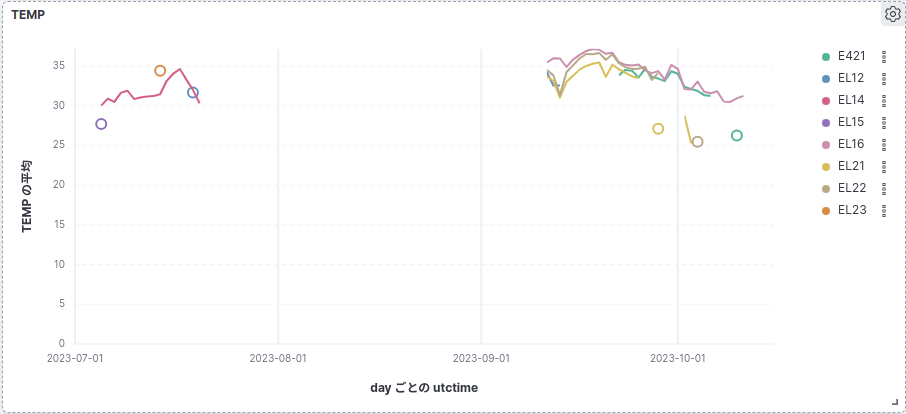
\includegraphics[width=160mm]{sotu/figure/co2Temp.png}
        \caption{co2インデックスのTEMP}
        \label{p24}
    \end{center}
\end{figure}

\begin{figure}[!ht]
    \begin{center}
        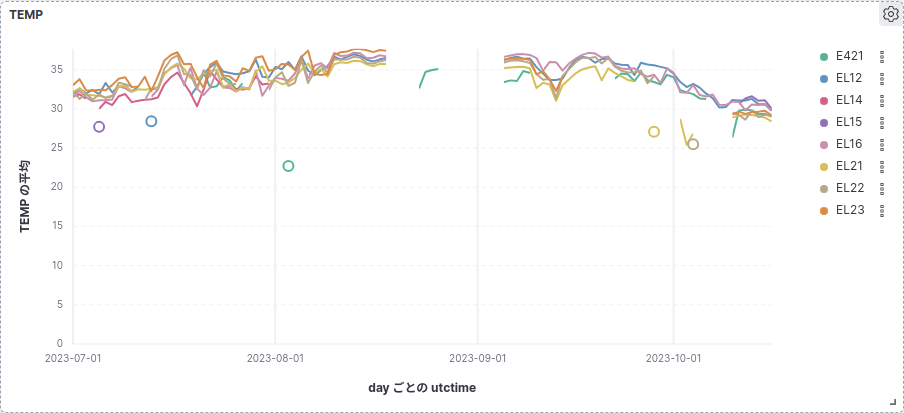
\includegraphics[width=160mm]{sotu/figure/co2ModbusTemp.png}
        \caption{co2\_modbusインデックスのTEMP}
        \label{p28}
    \end{center}
\end{figure}

\section{結言}
本章学内ゾーンにおける Elasticsearch クラスタへの
データ移行について述べた。

次章ではサーバーゾーンでのクラスタ構築における仮
想環境を使用した事前検証について述べる。